\section{Begriffe \& Definitionen} % (fold)
\label{sec:definitionen}

\subsection{Lernen} % (fold)
\label{sub:lernen}
\begin{quote}„Learning through personal experience and knowledge, which propagates from generation to generation, is at the heart of human intelligence. Also, at the heart of any scientific field lies the development of models (often, they are called theories) in order to explain the available experimental evidence at each time period. In other words, we always learn from data. Different data and different focuses on the data give rise to different scientific disciplines.“\footnote{\cite{mlearning}, Abschnitt „1.1 What Machine Learning is About“}
\end{quote}

\begin{quote}„Lernen im Sinne von Wissenserwerb kann als der Aufbau und die fortlaufende Modifikation von Wissensrepräsentationen definiert werden. [Es] ist ein bereichsspezifischer, komplexer und mehrstufiger Prozess, der die Teilprozesse des Verstehens, Speicherns und Abrufens einschließt […] und der auch zum Gebrauch – dem so genannten Transfer – des erworbenen Wissens führen kann.“\footnote{\cite{steiner}, Seite 163}
\end{quote}

Den obigen Zitaten zu Folge geschieht Lernen durch Erfahrung, durch Weitergabe von Wissen sowie durch die Interpretation von Daten. Diese können durch den Lernprozess zu Information und Wissen werden. Im Lernprozess sind sowohl die Lehrenden als auch die Lernenden aktiv handelnde Personen. Manche Teilprozesse können von einem Individuum bzw. von einem Paar aus Lehrer und Lerner, alle beschriebenen Teilprozesse können aber auch in Zusammenarbeit von Gruppen, auch mit wechselnden Rollen durchgeführt werden.
% subsection lernen (end)

\subsection{E-Learning} % (fold)
\label{sub:e_learning}
Unter \buzz{E–Learning} versteht man die Aneignung von Wissen mit elektronischen Medien.\footnote{vgl. \cite{gabler:elearning}} Oft werden unter dem Begriff multimediale, interaktive Lernsysteme wie Lernsoftware, Multimedia–Umgebungen, Simulationen beschrieben.\footnote{vgl. z.B. \cite{schulmeister} oder auch \cite{euler}} Solche Systeme sind i.d.R. an einzelne Lernende gerichtet, eine eventuelle Interaktion findet zwischen den Lernenden und dem Computersystem statt.
% subsection e_learning (end)

\subsection{Computer-supported collaborative learning} % (fold)
\label{sub:cscl}
Der Begriff \buzz{\ac{CSCL}} betont den Aspekt des \buzz{E–Learning by collaborating}, also der Zusammenarbeit von Lernenden untereinander sowie die zwischen Lernenden und Lehrenden.\footnote{vgl. \cite{euler:boos}, Seite 285} Hierbei kommen unterschiedliche Definitionen des Begriffs zum Einsatz. So wird das zweite „C“ je nach Schwerpunkt als „collaborative“, „cooperatove“, „collective“, „competitive“, oder auch „conversational” verstanden.\footnote{vgl. \cite{csclcomp}, Seite 1} 

Wie in einem traditionellen Klassenzimmer werden beim \ac{CSCL} somit bekannte pädagogische Konzepte Präsentation, Unterrichtsgespräch, Gruppenarbeit und das Gespräch zwischen Lernenden über Computernetzwerke hinweg umgesetzt. Aufgrund der Umsetzung im Netzwerk lassen sich hierbei jedoch Lerngruppen bilden, an denen deutlich mehr Personen Teilnehmen, als in einem Zimmer oder Auditorium Platz haben.

Die Interaktion findet beim \ac{CSCL} zwischen den beteiligten Menschen statt. Hierbei verschwimmen die Rollen von Lehrenden und Lernenden. Denn durch die Bearbeitung und Beantwortung der Fragen von Mit–Lernenden, wird die eigene Erkenntnis nicht nur an den Fragesteller weitergegeben, sondern auch beim Antwortenden vertieft und gefestigt. 


In Teilen der Literatur wird E–Learning als Bestandteil von \ac{CSCL} genannt. In dieser Arbeit soll jedoch das Augenmerk auf der Interaktion der Teilnehmer untereinander liegen, weshalb die Begriffe in der gegeneinander abgegrenzten Definitionen genutzt werden.
% subsection cscl (end)

\subsection{Online Campus Portal} % (fold)
\label{sub:online_campus_portal}
Im \buzz{\ac{OCP}} einer Hochschule\footnote{auch \ac{OCS}} werden die unterschiedlichen akademischen und organisatorischen Komponenten zusammengeführt. Verwaltung, Lehrende und Lernende können hier in entsprechenden Sichten auf die jeweils relevanten Funktionen zugreifen. Hierzu gehören die Bereitstellung von Informationen rund um das Studium, Prüfungsan– und Abmeldung, Notenbekanntgabe, Erstellung von Bescheinigungen und ähnliches. Für diese Arbeit besonders relevant sind die Teilsysteme \buzz{Benutzerverwaltung} sowie die elekronische Umsetzung der \buzz{Studien– und Prüfungsordnung} anhand derer die Zuordnung der Lernenden zu den Studienmodulen getätigt wird.\footnote{vgl. \cite{akad:campus}, 0'19" bis 3'55"}

Interaktion kann wie in Tabelle~\ref{tab:ocpinteractive} gezeigt in verschiedenen Ausprägungen auftreten:

\begin{table}[h]
\begin{tabular}{|l|l|m{4cm}|m{4cm}|}
\hline 
\multicolumn{2}{|l|}{\multirow{2}{*}{Interaktion im OCP}}                  & \multicolumn{2}{c|}{Empfänger}                                                                                 \\ \cline{3-4} 
\multicolumn{2}{|l|}{}                                   & \multicolumn{1}{c|}{Mensch}                                             & \multicolumn{1}{c|}{Programm}        \\ \hline
\multicolumn{1}{|c|}{\multirow{2}{*}{Sender}} & Mensch   & z.B. Versenden von Nachrichten an andere Studierende                    & z.B. An– und Abmeldung von Seminaren \\ \cline{2-4} 
\multicolumn{1}{|c|}{}                        & Programm & z.B. Mitteilung über zu Ende gehende Bearbeitungszeit eines Assignments & Interner Vorgang, keine vom Nutzer wahrgenommene Interaktion  \\ \hline
\end{tabular}
\caption{Interaktion im OCP}
\label{tab:ocpinteractive}
\end{table}

% subsection online_campus_portal (end)

\subsection{Fernhochschule} % (fold)
\label{sub:hochschule}

\begin{quote}
„Hochschule: Stätte für wissenschaftliche Forschung und Lehre, d.h. Weitergabe praktischer und theoretischer Kenntnisse in wissenschaftlicher Form an die Studierenden, an die bei Nachweis der erworbenen Kenntnisse und Fähigkeiten durch die vorgesehene Abschlussprüfung akademische Würden erteilt werden können.“
\footnote{\cite{gabler:hochschule}}\end{quote}

An einer Fernhochschule findet diese Weitergabe der Kenntnisse ausschließlich oder überwiegend in räumlicher Trennung von Lehrenden und Lernenden statt.\footnote{vgl. FernUSG, §1}
% subsection hochschule (end)


\subsection{Kommunikation} % (fold)
\label{sub:kommunikation}
Kommunikation wird von \cite{shannonweaver} als Informationsübertragung beschrieben, die Zwischen einer Quelle  und einem Empfänger\footnote{In der Orginalskizze vom „Receiver“ also „Empfänger” und der „Destination“, also Ebenfalls „Empfänger” gesprochen. Aufgrund der Doppeldeutigkeit im Deutschen wird der „Receiver“ in dieser Arbeit stets als „Dekodierer“ bezeichnet.} mit Hilfe eines Übertragungsmediums stattfindet. Vor der Übertragung werden die Informationen vom Sender kodiert und nach der Übertragung vom Empfänger dekodiert.\footnote{vgl. \cite{shannonweaver}, Seite 34} Während im ursprünglichen, technischen Modell Störungen lediglich bei der Übertragung stattfinden, wurde das Modell auf die Kommunikation zwischen Menschen erweitert, bei der auch bei der Kodierung und Dekodierung Fehler auftreten können.

Bei der Kommunikation zwischen Menschen wird somit nach diesem Modell die Botschaft in Worte kodiert, akkustisch oder schriftlich übertragen, und anschließend wieder vom Empfänger dekodiert. Da bei schriftlicher Kommunikation im Vergleich zum persönlichen Gespräch Details wie Betonung und Gesichtsausdruck, Körperhaltung, etc. nicht übermittelt werden, besteht auch hier beim Kodieren und Dekodieren erhöhtes Fehlerpotential.\footnote{vgl. \cite{rothe}, Seite 10f}

Die Kommunikation lässt sich nach den Dimensionen Synchronität, Senderzahl \& Empfängerzahl und Symmetrie des Wissensniveaus differenzieren. Diese Aspekte sowie der Betreuungsgrad, die Dauer des Bestehens der Lerngruppe, die Ziele welche erreicht werden sollen sowie die Zielgruppe (z.B. nach Alter oder vorhandenem Bildungsstand) bestimmen das konkrete Szenario, für welches die passenden Konzepte, Methoden und Werkzeuge gewählt werden müssen. \footnote{vgl. \cite{csclcomp}, Seite 3}

Aufgrund der schnellen Übertragung über das Internet ist die Synchronität nicht nur durch die gewählte Kommunikationsform, sondern durch die Verfügbarkeit der Kommunikationspartner und die Möglichkeit der  Zwischenspeicherung festgelegt. Durch schnelle Benutzerreaktion können eigentlich asynchrone Kommunikationsformen quasi synchron genutzt werden und umgekehrt. In dieser Arbeit sollen Kommunikationsformen als synchron angesehen werden, die ein schnelles Hin-- und Her von Nachrichten zwischen den Teilnehmern fördert, wie z.B. (Video--)Telefonie oder Chatsysteme. Asynchron werden dahingegen die Kommunikationsformen bezsichnet, welche i.d.R. so genutzt werden, bzw. die Aufgrund Ihrer Struktur eine Form des Austauschs fördern, die durch längere oder länger durchdachte Beiträge charakterisiert wird, wie z.B. E--Mail oder Forenbeiträge.

% subsection kommunikation (end)

\subsection{Daten, Information, Wissen}
\label{sub:defwissen}

In dieser Arbeit sollen die folgenden Definitionen gelten: Ein \buzz{Datum} ist eine formalisierte Sachverhaltsaussage, ohne inhärente Bedeutung (z.B. „23°C“). Durch Interpretation im Kontext kann daraus eine \buzz{Information} werden (z.B. „Die Außentemperatur beträgt 23°C“).\footnote{vgl. \cite{kfk}, Seite 40} Durch Vernetzung mehrerer Informationen miteinander, aber auch durch Erfahrung kann \buzz{informatives Wissen} entstehen (z.B. „Das Wetter ist schön“).\footnote{vgl. \cite{pnik}, Seite 106}

In weiteren Verfeinerungsschritten entsteht dann \buzz{handlungsorientiertes Wissen}, (z.B. „Ich benötige beim Nachmittagsspaziergang keinen Pullover“) das dann zu einer konkreten Entscheidung führen kann (z.B. „Ich lasse den Pullover zu Hause.“).\footnote{vgl. \cite{taylor}, Seite 342}

\subsection{Web 1.0, Web 2.0}

Unter \buzz{Web 1.0} versteht man das \buzz{\ac{WWW}} wie es ursprünglich entwickelt wurde: Eine Menge von statischen Daten, die miteinander auf willkürliche Weise verknüpft werden konnten. Die Auszeichnungssprache \buzz{\ac{HTML}} ermöglicht es Autoren, bestimmte Abschnitte zu kennzeichnen. Schon hier gibt es unterschiedliche Informationsstufen der Auszeichnungen: Während \code{<b>…</b>} lediglich aussagt, dass der ausgezeichnete Abschnitt in fetter Schriftart angezeigt werden soll, ist eine mit \code{<h1>…</h1>} ausgezeichnete Überschrift tatsächlich als solche zu erkennen. Auch wenn die dadurch gewonnene Information für ein automatisch erstelltes Inhaltsverzeichnis schon nützlich sein kann, wird hier keine Aussage bzgl. des eigentlichen Inhalts getroffen. Somit sind die Dokumente des Web 1.0 dem Bereich der \buzz{Daten}\index{Daten} zuzuordnen. Darin enthalten Information bzw. in einem solchen Hypertextsystem enthaltenes Wissen ist erst zugänglich, wenn diese von Menschen gelesen und ausgewertet werden.\footnote{vgl. \cite{alkhatib}, Seite xvi} 

Die Daten des \buzz{Web 2.0} werden i.d.R. in Datenbanken vorgehalten und die Webseiten erst bei Abruf generiert. Durch die Popularität von Werkzeugen wie Blogs und Wikis sind deutlich mehr Menschen an der Erstellung der Inhalte beteiligt. Diese werden auch mit sogenannten \buzz{Meta--Daten} angereichert. Hierdurch wird in maschinenlesbarer Form angegeben, welche Informationen die Dokumente enthalten. Neben vom Autor selbst zugeordneten \buzz{Taxonomien} kommen auch automatisch generierte Meta--Daten hinzu. Beispiele hierfür sind etwa das Veröffentlichungsdatum, Beziehungen zu anderen Dokumenten\footnote{Realisiert durch sog. Backtracks -- „Wer verlinkt auf dieses Dokument?“} oder Geoinformationen („Wo wurde das Dokument erstellt?“). Inzwischen werden auch die Stimmung des Autors erfragt (z.B. bei Runtastic–Aktivitäten bzw. Facebook--Einträgen) oder durch Textanalyse ermittelt (z.B. bei der Auswertung von Produktrezessionen\footnote{vgl. \cite{sprejz}, Seite 11ff}). Die durch Daten und Meta--Daten erzielte Informationsstufe ist deutlich über der von \buzz{Web 1.0} einzuordnen, unterliegt aber je nach genutzter Software bzw. Nutzereingaben deutlichen Schwankungen.

Das \buzz{Web 2.0} ist durch einen hohen Grad an Interaktivität gelennzeichnet. Die Einstiegshürden sind niedrig, so dass durch Kommentar bzw. Antwortfunktionen oder auch durch die Möglichkeit selbst Beiträge zu erstellen jeder Nutzer auch zum Produzierenden werden kann. Diese Eigenschaft bewirkt dass die Werkzeuge des \buzz{Web 2.0} sich für die Nutzung in \buzz{\ac{CSCL}--Umgebungen} empfehlen.\footnote{vgl. \cite{livingston}, Abschnitt „Web 2.0 and blended learning“}

\subsection{Web 3.0 = Web 2.0 + Semantik = Semantisches Web}

\begin{quote}„\buzz{Semantik}, auch \buzz{Bedeutungslehre}, nennt man die Theorie oder Wissenschaft von der Bedeutung der Zeichen. Zeichen können in diesem Fall Wörter, Phrasen oder Symbole sein. Die Semantik beschäftigt sich typischerweise mit den Beziehungen zwischen den Zeichen und den Bedeutungen dieser Zeichen.“\footnote{\cite{wp:semantik}}\end{quote}

\begin{quote}„Semantics is the process of communicating enough meaning to result in an action. A sequence of symbols can be used to communicate meaning, and this communication can then affect behavior.“\footnote{\cite{sagaran}, Abschnitt „1. Why Semantics?“}\end{quote}

Im \buzz{Web 3.0} werden die Daten bzw. Informationen des Web 2.0 durch Beifügung von Bedeutung zu Information bzw. informativem Wissen veredelt\footnote{vgl. \cite{nyt:markoff}}. Hierdurch soll es den Lernenden ermöglicht werden, die gesammelten Datenmengen sinnvoll zu nutzen\footnote{vgl. \cite{tsp:tolksdorf}}. Wenn wie in \cite{sagaran} beschrieben eine Datensequenz ausreichend Bedeutung transportiert, dass dadurch Verhalten\footnote{sowohl das Verhalten von Menschen als auch das von Programmen} beeinflusst werden kann, dann kann diese als \buzz{handlungsorientiertes Wissen}\footnote{siehe Abschnitt~\myref{sub:defwissen}} betrachtet werden.

Die Bezeichnung \buzz{semantisches Web} ermöglicht eine Abgrenzung gegenüber anderen Interpretationen des Begriffs \buzz{Web 3.0}, wie sie z.T. im Marketing\footnote{z.B. „Web 3.0 marketing is the convergence of new technologies and rapidly changing consumer buying trends.“ in \cite{web3market}, Abschnitt „What is Web 3.0 Marketing?“} oder in der Politikwissenschaft\footnote{z.B. „Is this Web 3.0? Not a tech-upgrade, a smarter algorithm, slicker fibre optic or better Bluetooth beam. Instead, Web 3.0 as in an outcome, the demonstrated consequences of being able to access information?“ in \cite{web3pol}, Abschnitt „Web 3.0: Regime Change“} zu finden sind.

% section definitionen (end)

\newpage
\section{Werkzeuge des CSCL} % (fold)
\label{sec:werkzeuge_des_cscl}

\subsection{Materialien zum Selbststudium} % (fold)
\label{sub:materialien_zum_selbststudium}
Die von der Fernhochschule zur Verfügung gestellten Lernmaterialien bzw. die in den Modulbeschreibung aufgeführte Literatur bildet das konkrete Wissensfundament auf Themenebene und definieren den im jeweiligen Modul zu lernenden Stoff.\footnote{vgl. \cite{pnikmail}} Hierdurch wird auch festgelegt, ob Beiträge, die in den anderen Werkzeugen veröffentlicht werden themenrelevant sind oder nicht.
% subsection materialien_zum_selbststudium (end)

\subsection{Audio– und Video–Vorlesungen} % (fold)
\label{sub:audio_und_video_vorlesungen}
Die Lehrveranstaltungen werden hier über das Internet als Videostream oder Audio–Podcast den Lernenden zur Verfügung gestellt. Rückmeldung kann hierbei entweder in der jeweiligen Software vorgesehen sein (z.B. bei \buzz{Adobe Connect}, \buzz{Skype}) oder über einen separaten Kanal wie z.B. \buzz{Twitter} erfolgen. Diese Online–Veranstaltungen stellen aufgrund der meist beschränkten Möglichkeit zur Rückmeldung eine synchrone Eins-zu-Viele-Kommunikation dar. Durch Aufzeichnung der Veranstaltung können diese ganz oder Teilweise den Lernenden auch dauerhaft als Lernvideos oder Lernpodcasts zur Verfügung gestellt werden.\footnote{z.B. \buzz{iTunes U} oder \url{youtu.be/iSWchj8hSFA}} Hierbei ist zu beachten, dass falls es sich hierbei um Aufnahmen von Veranstaltungen mit Publikum handelt, diese damit einverstanden sein müssen, evt. in den Videos erkennbar zu sein.\footnote{vgl. \cite{cs50}, ab 15'07" }
% subsection audio_und_video_vorlesungen (end)

\subsection{Forensysteme} % (fold)
\label{sub:forensysteme}
Bei \buzz{Online--Foren} handelt es sich um Systeme mit deren Hilfe die beliebig viele Nutzer selbst gewählte Themen asynchron diskutieren können. Die Themen sind meist in Themenbereich bzw. Unterforen gegliedert. Eine Einstufung der Nutzer aufgrund der bereits verfassten Beiträge ist üblich, durch regelmäßig Nutzung kann also eine Reputation aufgebaut werden. Moderatoren können für Themenbereiche oder das gesamte Forum bestimmt werden, die neben der Konfiguration der Themenstruktur im Bedarfsfall auch die Möglichkeit haben, die Beiträge anderer Nutzer zu bearbeiten oder Benutzerkonten zu sperren. Die Forenbeiträge sind i.d.R. für alle Nutzer sichtbar. Benutzer können Themen abonnieren oder sich die seit dem letzen Besuch neu hinzugekommenen Beiträge anzeigen lassen, womit die Interaktion gefördert wird.\footnote{vgl. \cite{vbulletin}, Abschnitt „What is a community bulletin board?“}
% subsection forensysteme (end)

\subsection{Trouble–Ticket–Systeme} % (fold)
\label{sub:trouble_ticket_systmee}
Bei einem \buzz{\ac{TTS}} handelt es sich um ein Nachrichtensystem, das Benutzeranforderungen wie etwa Supportanfragen entgegennimmt und diese einem Betreuungsteam zur Verfügung stellt. Die Anfragen können dann von beliebigen Teammitgliedern beantwortet, gekennzeichnet oder an Spezialisten weitergeleitet werden. Die Antwort wird dann über das System an den Fragesteller zurück übermittelt. Durch entsprechende Kennzeichnungen können noch offene Anfragen schnell erkannt werden. Durch das \ac{TTS} soll sichergestellt werden, dass keine Resourcen verschwendet wird und trotzdem keine Supportanfrage unbeantwortet bleibt.\footnote{\cite{nna}, Abschnitt „12.4. Reporting Bugs via Bugzilla“} Im Kundensupport sind diese Systeme eigenständig und für die Kunden sichtbar. Im hier vorgestellten Konzept nehmen sie jedoch eine für Lernende unsichtbare Hilfsfunktion ein, die den Dozenten bei der Überwachung der Forenbeiträge helfen soll.
% subsection trouble_ticket_systmee (end)

\subsection{Wikis} % (fold)
\label{sub:wikis}
Ein \buzz{Wiki} ist ein Schreibsysteme, bei dem Nutzer gemeinsam an Dokumenten arbeiten können. Neue Wiki--Seiten lassen sich schnell und einfach erstellen und sind i.d.R. für alle Nutzer sichtbar. Die Bearbeitung steht allen Teilnehmern offen. Zu den grundlegenden Funktionen gehört ein einfacher Markup--Syntax oder ein \ac{WYSIWYG} Editor für \ac{HTML}, eine Versionsverwaltung um Bearbeitungen nachvollziehen und bei Bedarf rückgängig machen zu können, die Auflistung von kürzlich bearbeiteten Seiten. Einzelne Seiten oder Themenbereiche können abonniert werden. Die ersten Wiki--Systeme waren ohne jegliche Benutzerhierarchie, inzwischen ist jedoch eine Nutzerverwaltung und Rollenverteilung üblich.\footnote{vgl. \cite{cscl:ebner}, Seite 103f} Meist gibt es für Wikis keine oder nur sehr lockere redaktionelle Vorgaben, um möglichst viele Nutzer zur Mitarbeit zu motivieren. Hierdurch, in Kombination mit der Versionsverwaltung, eignen sich Wikis gut für die gemeinsame, kontinuierliche Erarbeitung von Dokumenten.\footnote{vgl. \cite{cunningham}, Abschnitt „Why Wiki?“}

Eine spezielle Form von Wikis\footnote{z.B. \buzz{Etherpad}, siehe \url{etherpad.org}} erlauben die gleichzeitige Bearbeitung der Seiten durch mehrere Benutzer.
% subsection wikis (end)

\subsection{Wissensbasis} % (fold)
\label{sub:knowledge_bases}
In einer \buzz{Wissensbasis}\footnote{engl. Knowledge–Base; der deutsche Begriff \buzz{Wissens--Datenbank} soll hier aufgrund des Wiederspruchs, \buzz{Wissen} in einer \buzz{Datenbank} zu speichern vermieden werden. Der Begriff \buzz{Wissensbank} hat sich in der Literatur nicht durchgesetzt.} werden Dokumente gesammelt, die häufig wiederkehrende oder grundlegende Themen ausführlich besprechen. In ihr ist explizites Wissen schriftlich gesammelt.\footnote{vgl. \cite{wp:kb}} Die hier verfügbaren Dokumente sind redaktionell erstellt und können Informationen aus  anderen Kommunikationsmitteln zusammenfassen, verdichten und vertiefen. Das beschriebene Thema oder Teil–Thema sollte umfassend besprochen werden. Die eingesetzte Software kann ein Wiki--System sein, jedoch ist die Herangehensweise formeller, um die gewünschte Qualität sicherstellen zu können. 

Das Ziel der Wissensbasis ist es, das benötigte Wissen zum richtigen Zeitpunkt und im richtigen Umfang zur Verfügung zu stellen.
Das Auffinden von relevanten Dokumenten ist eine grundlegende Funktion jeder Knowledge–Base und kann durch Volltextsuche, einer Themenhierarchie in Baumstruktur und/oder durch Taxonomien zur Beschreibung des Inhalts geschehen.\footnote{vgl. \cite{altwies}, Abschnitt „Corporate Knowledge Base“} 

% subsection knowledge_bases (end)

\subsection{Persönliche Kommunikationsmittel} % (fold)
\label{sub:personliche_kommunikationsmittel}
Den einzelnen Teilnehmern einer Lerngruppe stehen des Weiteren alle Möglichkeiten der individuellen Kommunikation zur Verfügung. Hierzu sind aufgrund der Popularität die synchronen textbasierten Chatsysteme (Whatsapp, Facebook Messenger, proprietäre Funktionen des \ac{OCS}) sowie Skype mit der Möglichkeit von Audio– oder Video–Konferenzen für kleine Gruppen zu zählen. Für asynchronen Nachrichtenaustausch bietet sich E–Mail an. Bei der Nutzung der Individuellen Kommunikation kann Vertraulichkeit gewahrt werden, jedoch stehen die Möglichkeiten der anderen Werkzeuge nur beschränkt zur Verfügung. 
% subsection personliche_kommunikationsmittel (end)

\subsection{Prüfungsleistung} % (fold)
\label{sub:prufungsleistung}
Die Prüfungsleistung in Form einer Klausur oder eines Assignments bildet den Abschluss der Lernanstrengung des jeweiligen Moduls und dient somit als Möglichkeit der Erfolgskontrolle für den Lernprozess.
% subsection prufungsleistung (end)

\subsection{Zusammenspiel der Werkzeuge} % (fold)
\label{sub:zusammenspiel_der_werkzeuge}
Die Video– bzw. Audio–Vorlesungen bilden zusammen mit den sonstigen Lernmaterialien das Fundament für den gemeinschaftlichen Teil des Lernprozesses. Fragen, Probleme oder Anmerkungen zum Lernstoff können dann von den Lernenden im entsprechenden Forum veröffentlicht und von anderen Teilnehmern der Lerngruppe oder vom Dozenten werden. Das \ac{TTS} unterstützt die Dozenten dabei, dass keine Forenbeiträge unbeantwortet bleiben.
Themen, die eine intensiveren Bearbeitung notwendig haben, werden von Teilnehmern der Lerngruppe auf Wiki–Seiten übertragen, welche dann wiederum von der Gemeinschaft bearbeitet, strukturiert und verfeinert werden. Ab einem zu bestimmenden Reifegrad können Wiki–Seiten oder Teile davon in die Wissensbasis und anschließend in die Lernmaterialien integriert werden. Dieser Prozess muss klar definiert sein, um die Qualität sicherstellen zu können. 

\begin{figure}[H]
\begin{center}
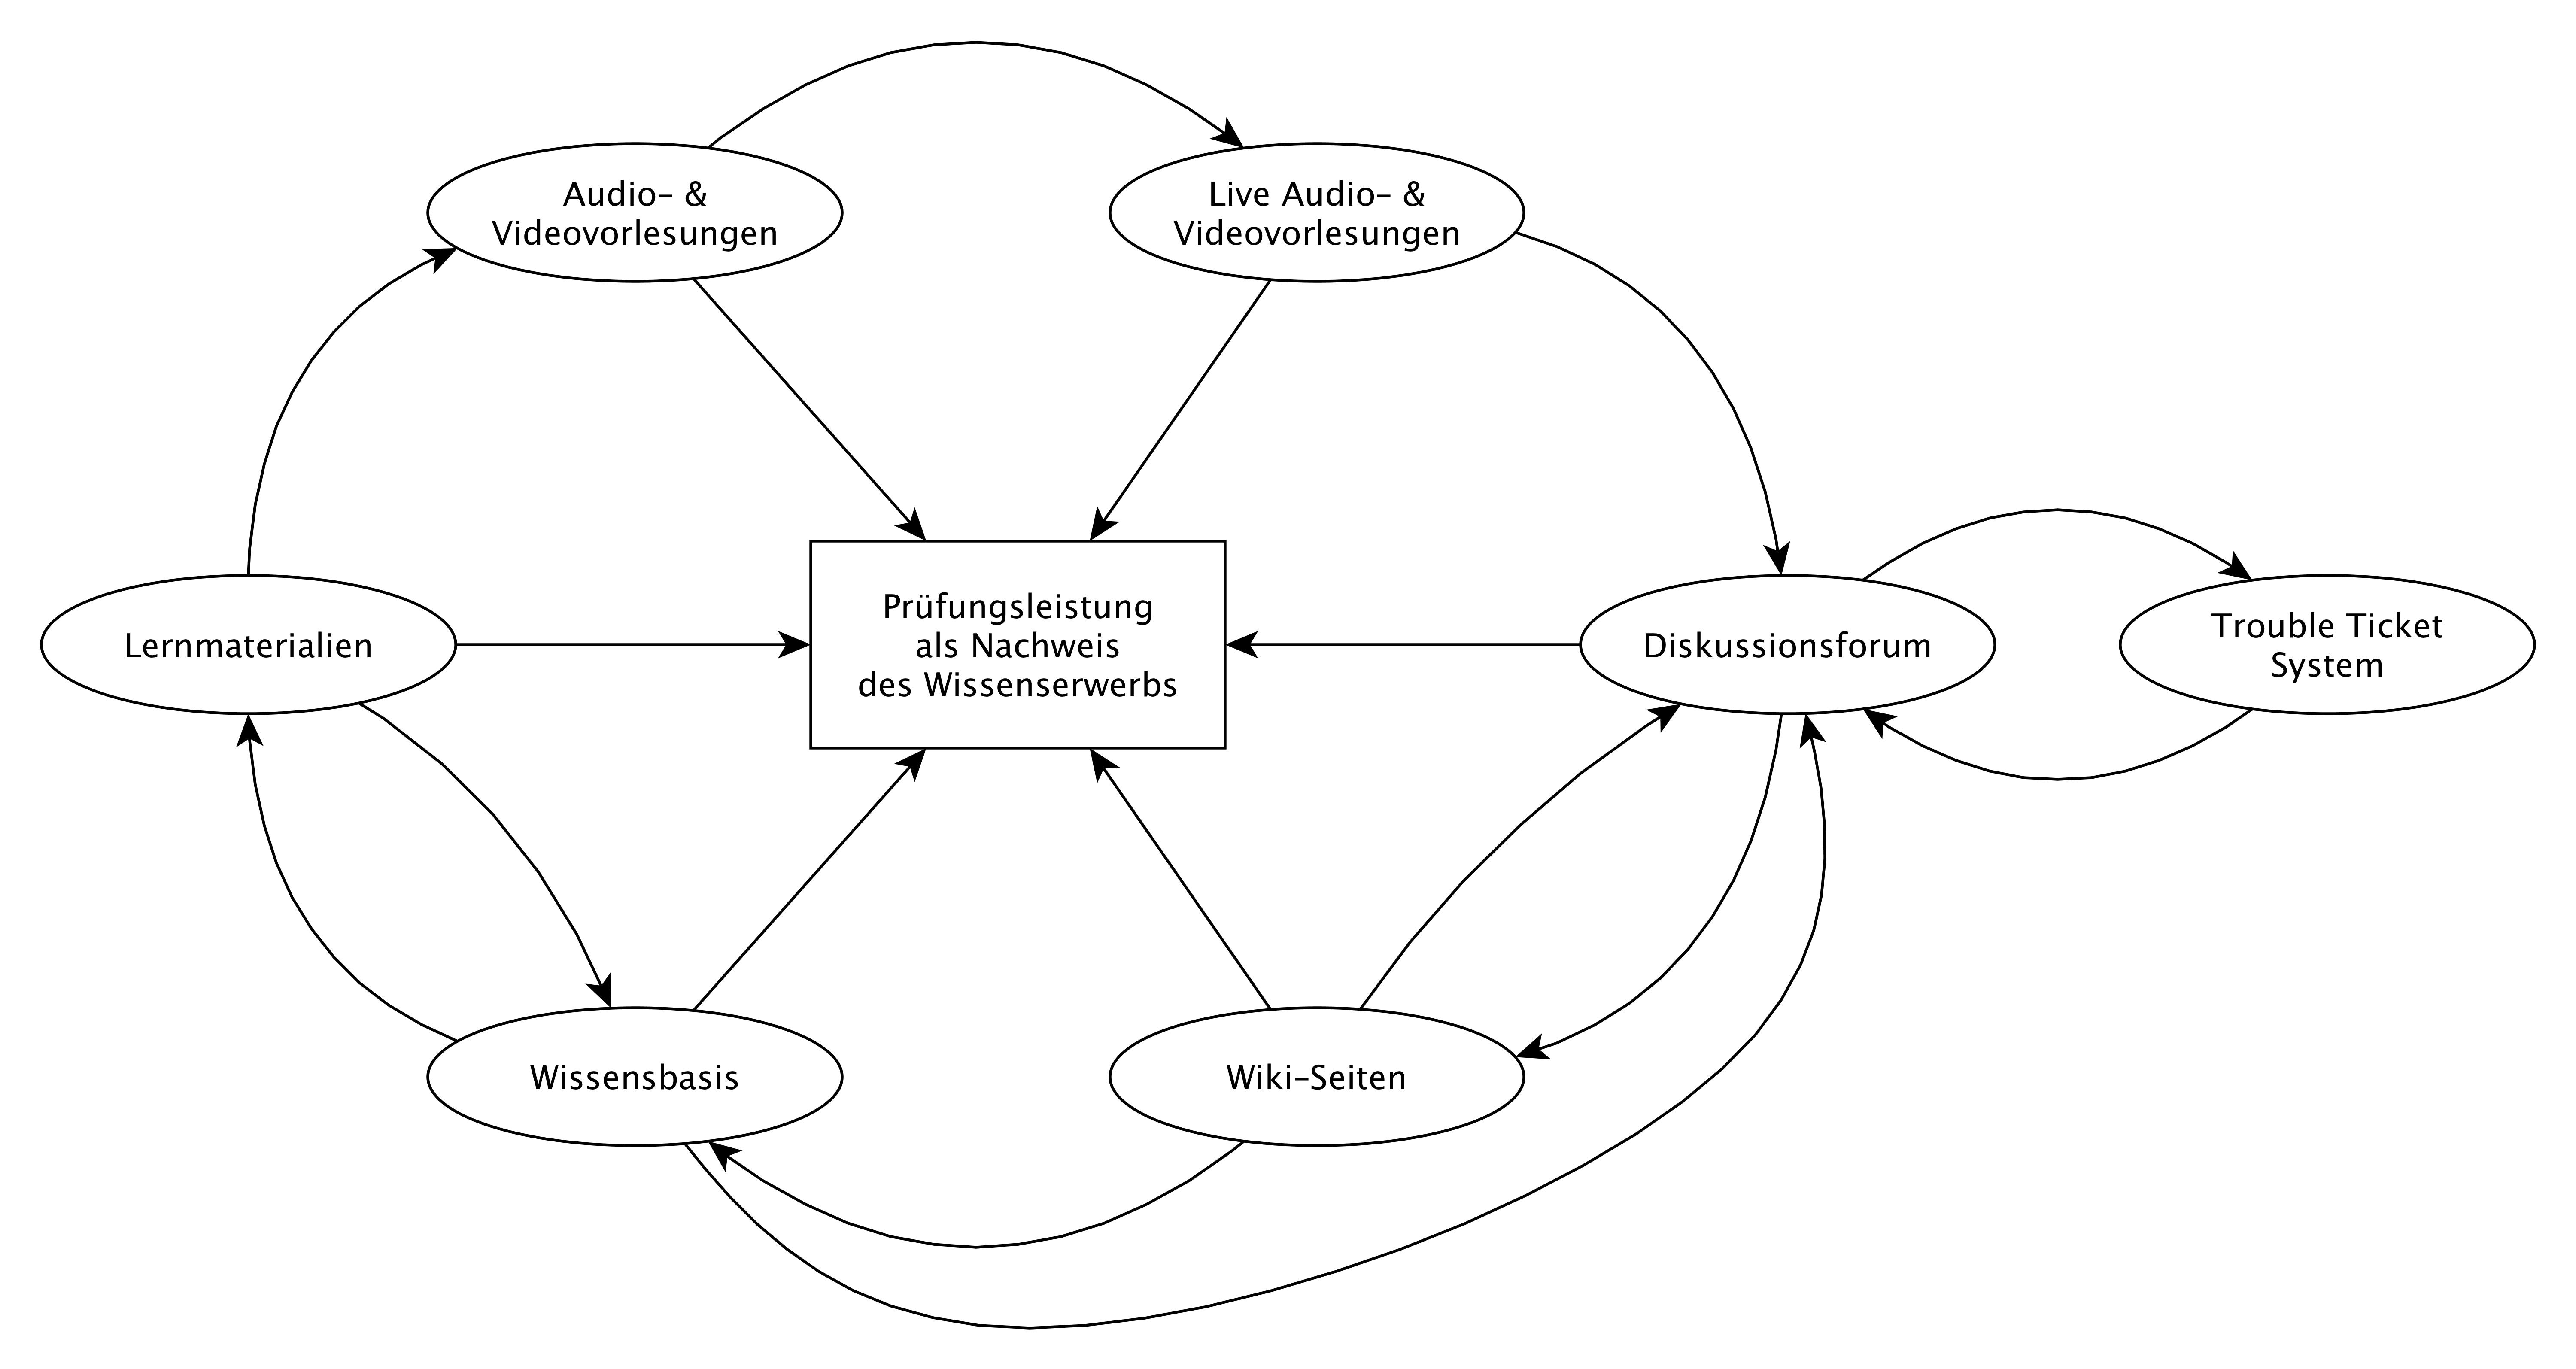
\includegraphics[width=\textwidth]{tools.jpg}
\caption{Zusammenspiel der CSCL–Werkzeuge}
\label{fig:toos}
\end{center}
\end{figure}

Unabhängig von diesem idealen Ablauf, können Beiträge aller genutzten Werkzeuge jeweils zur Verbesserung der jeweils anderen genutzt werden. So können Forenbeiträge in einer Video–Vorlesung thematisiert werden, oder eine Wiki–Seite wird zur Beantwortung einer Frage im Forum zitiert. Ein erfolgreicher Lernprozess wird durch das Bestehen der Prüfungsleistung offiziell bestätigt.
% subsection zusammenspiel_der_werkzeuge (end)

\subsection{Lizenzen} % (fold)
\label{sub:lizenzen}
Um die in Abschnitt~\myref{sub:zusammenspiel_der_werkzeuge} beschriebenen Vorgänge des Kopierens, Anpassens, Verfeinerns und Adaptierens möglich zu machen, müssen alle Teilnehmer ihre Beiträge unter eine gemeinsame Lizenz stellen. Diese Lizenz muss das Kopieren und Verändern, zumindest innerhalb der \ac{CSCL}–Umgebung erlauben. Da durch den gemeinschaftlichen Lernprozess auch die Materialien zum Selbststudium optimiert werden, sollte diese Lizenz eine kommerzielle Nutzung einschließen. 

Eine Klausel, dass abgeleitete Werke unter eben dieser Lizenz stehen müssen, kann die Motivation zur Mitarbeit erhöhen, wenn den Beteiligten erklärt wird, dass ihre Beiträge dadurch zwar von allen genutzt, aber von niemandem „weggenommen“ werden können. Die Lizenz \buzz{\ac{CC-by}}\footnote{siehe \url{creativecommons.org/licenses/by/4.0/}} ist ein Beispiel für eine Lizenz, welche die genannten Anforderungen erfüllt.\footnote{vgl. \cite{baraniuk}, ab 14'00"} Die \ac{CC-by} wird z.B. auch vom \buzz{Springer–Verlag} in deren Journals und auf der Plattform \buzz{SpringerLink} für OpenAccess–Veröffentlichungen verwendet\footnote{vgl. \cite{springercc}}, was die Bekanntheit innerhalb der Zielgruppe der akademischen Autoren erhöhen und Vorbehalte verringern sollte.
% subsection lizenzen (end)

% section werkzeuge_des_cscl (end)

\newpage
\section{Ziele} % (fold)
\label{sec:ziele}

\subsection{Zielgruppe} % (fold)
\label{sub:zielgruppe}
Die Hauptzielgruppe der Lernplattform sind die \buzz{Studierenden der Hochschule}. Die Studierenden bewegen sich frei im Lernstoff und wählen nach eigenen Vorlieben zwischen den CSCL–Werkzeugen. Ein besonderes Augenmerk sollte hier auf die Studierenden gelegt werden, die das jeweilige Modul bereits abgeschlossen haben, da von diesen zu erwarten ist, dass sie besonders wertvolle Beiträge und Lerntips im Diskussionsforum bereitstellen.\footnote{siehe z.B. \url{Fernstudenten.de}}

Die \buzz{Dozenten}\footnote{inkl. der Autoren der Studienmaterialien} und die \buzz{Studienbetreuung} bilden weitere Zielgruppen, die als Arbeitnehmer bzw. Dienstleister der Hochschule die Lernplattform als eines der Hauptwerkzeuge ihres regelmäßigen Kontakts zu den Studierenden erfahren. Auch wenn Gruppen die nur aus Studierenden bestehen gut funktionieren können, ist es ohne offizielle Stellungnahmen nicht möglich, bestimmte Sachverhalte abschließend zu klären.

Hochschulfremde Personen wie \buzz{Interessenten}, \buzz{Arbeitgeber von aktuellen oder potentiellen Studierenden} und \buzz{Studierende anderer Hochschulen} kommen mit Einschränkungen ebenfalls als Zielgruppen in Frage, da eine qualitativ hochwertige, transparente Lernplattform die Reputation der Hochschule verbessern kann.\footnote{siehe z.B. \cite{cs50}} 
% subsection zielgruppe (end)

\subsection{Zentrales Ziel: Wissenserwerb \& Studienabschluss} % (fold)
\label{sub:zentrales_ziel_wissenserwerb_studienabschluss}
Wie in der Definition in Abschnitt~\ref{sub:hochschule} und in Abbildung~\ref{fig:toos} auf Seite \pageref{fig:toos} ersichtlich wird, sind alle Aktivitäten auf das zentrale Ziel des Wissenserwerb bzw. auf den erfolgreichen Abschluss des Studienmoduls und letztendlich des Studiums ausgerichtet. Dieses Ziel steht nicht nur über den Anstrengungen im pädagogischen Bereich, sondern ist auch Leitlinie in allen anderen Bereichen. Eine Hochschule, die in diesem Kernbereich nicht erfolgreich ist, kann auch als ganzes nicht erfolgreich sein. Hierbei hat sowohl der Wissenstransfer als auch die zugehörigen Abschlussprüfungen wissenschaftlichen Ansprüchen genügen.
% subsection zentrales_ziel_wissenserwerb_studienabschluss (end)

\subsection{Pädagogische Ziele} % (fold)
\label{sub:padagogische_ziele}
Neben dem Wissenstransfer sollen die Studierenden die Prinzipien des wissenschaftlichen Arbeitens erlernen, einüben und nutzen. Durch gegenseitige Hilfestellung im Forum soll das Wissen sowohl beim Fragesteller als auch bei den Antwortenden vertieft werden. Durch die gemeinsame Arbeit in Forum und Wiki sollen die Studierenden Teamarbeit einüben. Durch die Zusammenarbeit von Lernenden und Lehrenden soll außerdem die Aktualität und Qualität der Studienmaterialien verbessert werden.
% subsection padagogische_ziele (end)

\subsection{Organisatorische Ziele} % (fold)
\label{sub:organisatorische_ziele}
Auf organisatorischer Ebene soll der Einsatz einer CSCL–Plattform den optimalen Einsatz der zur Verfügung stehenden personellen Mittel zur akademischen und organisatorischen Betreuung der Studierenden ermöglichen. Außerdem soll die Betreuungsqualität dadurch erhöht werden, dass Anfragen schneller abschließend beantwortet werden können. 

Ein weiteres Ziel ist, dass impliziertes Wissen expliziert, wie es z.B. beim Verfassen eines Forenbeitrags der Fall ist. Ebenfalls soll nach Möglichkeit individuellen Wissen, etwa durch die Integration Betreuungsprozesse, in organisatorisches Wissen überführt wird.\footnote{vgl. \cite{lws}, Seite 358}
% subsection organisatorische_ziele (end)

\subsection{Nutzerakzeptanz} % (fold)
\label{sub:nutzerakzeptanz}
Als Grad der Nutzerakzeptanz unter Studierenden kann das Verhältnis der über die CSCL–Plattform behandelten Anfragen zu denen über die klassischen Kanäle persönliche E–Mail oder Telefon behandelten Anfragen. Da sowohl Dozenten als auch die Studienbetreuung auf dem Kanal antworten sollten, der von den Studierenden gewählt wird, ist das Verhältnis CSCL zu klassisch bei diesen Zielgruppen keine geeignete Kennzahl. Über alle Zielgruppen hinweg kann die Anzahl der Nutzer die Fragen im Forum stellen, Nutzer die diese Beantworten, Nutzer die Wikiseiten erstellen und derer die diese editieren als Indikatoren für die Akzeptanz des Systems genutzt werden.
% subsection nutzerakzeptanz (end)

\subsection{Inhaltliche Qualität} % (fold)
\label{sub:inhaltliche_qualitat}
Die objektive Bewertung der inhaltichen Qualität der im Lernsystem vorhandenen Artikel ist äußerst schwierig. Als Maß für die Steigerung der inhaltlichen Qualität kann die Anzahl der aus Wiki bzw. Wissensbasis in die Studienmaterialien herangezogen werden. Um einfache Rechtschreibkorrekturen von Umfangreichen inhaltlichen Aktualisierungen unterscheiden zu können, bietet sich eine entsprechende Gewichtung, etwa nach geänderten Buchstaben oder nach Kategorien\footnote{z.B. Rechtschreibkorrektur: 1 Punkt, Aktualisierung von Daten ohne fachliche Änderung: 2 Punkte, Inhaltliche Korrekturen: 5 Punkte pro Absatz, etc.} an.
% subsection inhaltliche_qualitat (end)

\subsection{Zielkonflikt: Betreuungsqualität vs. Involvement} % (fold)
\label{sub:zielkonflikt_betreuungsqualitat_vs_involvement}
Der wohl größte Konflikt besteht wohl zwischen dem Anspruch, Anfragen der Studierenden möglichst schnell und kompetent zu bearbeiten und der Absicht, möglichst viele Studierende in die Lösungsfindung bei akademischen Fragen zu involvieren. Hier bedarf es ein System, nach dem Wichtigkeit, Dringlichkeit und pädagogisches Potential der Fragen zu bewerten sind, damit vom Dozenten entsprechend dieser Einordnung eine passende Antwortstrategie gewählt werden kann. 

Das in Abbildung~\ref{fig:wuerfel} gezeigte Schema ist eine 3-dimensionale Anpassung der von Covey beschriebenen Matrix zur Priorisierung von Aufgaben dar\footnote{vgl. \cite{covey}, Seite 6}.
%%%%%%%%%%%%%%%%%%%%%%%%%%%%%%%%%%%%%%%%%%%%%%%%%%%%%%%%%%%%%%%
%
% Welcome to Overleaf --- just edit your LaTeX on the left,
% and we'll compile it for you on the right. If you give
% someone the link to this page, they can edit at the same
% time. See the help menu above for more info. Enjoy!
%
% Note: you can export the pdf to see the result at full
% resolution.
%
%%%%%%%%%%%%%%%%%%%%%%%%%%%%%%%%%%%%%%%%%%%%%%%%%%%%%%%%%%%%%%%
% :Author: Stefan Kottwitz
% :Source: TeXblog - TikZ: shaded cube
%          http://texblog.net/latex-archive/graphics/tikz-cube-3d/
\begin{comment}

:Title: Sudoku 3D cube
:Tags: 3D, Transformations

This example shows how to create an effective 3D effect using the ``slant`` transformation.
Shading has been added to enhance the 3D impression. Read more about this example over
at TeXblog_. 

.. _TeXblog: http://texblog.net/latex-archive/graphics/tikz-cube-3d/

:Author: Stefan Kottwitz
:Source: `TeXblog - TikZ: shaded cube`__

.. __: http://texblog.net/latex-archive/graphics/tikz-cube-3d/

\end{comment}
\begin{figure}[bth]
\begin{center}
\begin{tikzpicture}[every node/.style={minimum size=1cm},on grid, scale=3]
\begin{scope}[every node/.append style={yslant=-0.5},yslant=-0.5]
%  \shade[right color=gray!10, left color=black!50] (0,0) rectangle +(2,2);
  \node at (0.5,1.6) {geringe};
  \node at (0.5,1.4) {Relevanz};
  \node at (1.5,1.6) {hohe};
  \node at (1.5,1.4) {Relevanz};
  \node at (0.5,0.6) {geringe};
  \node at (0.5,0.4) {Relevanz};
  \node at (1.5,0.6) {hohe};
  \node at (1.5,0.4) {Relevanz};
  \draw (0,0) grid (2,2);
\end{scope}
\begin{scope}[every node/.append style={yslant=0.5},yslant=0.5]
%  \shade[right color=gray!70,left color=gray!10] (2,-2) rectangle +(2,2);
  \node at (2.5,-0.4) {hohes};
  \node at (2.5,-0.6) {Potential};
  \node at (3.5,-0.4) {hohes};
  \node at (3.5,-0.6) {Potential};
  \node at (2.5,-1.4) {geringes};
  \node at (2.5,-1.6) {Potential};
  \node at (3.5,-1.4) {geringes};
  \node at (3.5,-1.6) {Potential};
  \draw (2,-2) grid (4,0);
\end{scope}
\begin{scope}[every node/.append style={
    yslant=0.5,xslant=-1},yslant=0.5,xslant=-1
  ]
 % \shade[bottom color=gray!10, top color=black!80] (4,2) rectangle +(-2,-2);
  \node at (2.5,1.6) {hohe};
  \node at (2.5,1.4) {Dringlichkeit};
  \node at (2.5,0.6) {hohe};
  \node at (2.5,0.4) {Dringlichkeit};
  \node at (3.5,1.6) {geringe};
  \node at (3.5,1.4) {Dringlichkeit};
  \node at (3.5,0.6) {geringe};
  \node at (3.5,0.4) {Dringlichkeit};
  \draw (2,0) grid (4,2);
\end{scope}
\end{tikzpicture}
\caption{Einteilung der Forenbeiträge}
\label{fig:wuerfel}
\end{center}
\end{figure}

Diese Einteilung kann durch Vergabe von entsprechenden Merkmalen durch die Nutzer (Fragestellern und Kommilitonen) oder durch automatische Erkennung von Schlüsselworten geschehen.

Von den acht möglichen Einstufungen sind die folgenden besonders Beachtenswert:

\begin{itemize}
	\item \textbf{Dringlichkeit: Hoch, pädagogisches Potential: Hoch, Themenrelevanz: Hoch}\\
				Hier besteht der Interessenskonflikt zwischen der Notwendigkeit eine dringende, relevante Anfrage schnell durch einen Dozenten zu beantworten, 
				und der Realisierung des pädagogischen Potentials durch einen eventuell lange dauernde Diskussion in der Lerngruppe. 
				Dieser Konflikt könnte evt. durch eine private Nachricht vom Dozenten an den Fragesteller mit anschließender öffentlicher Diskussion gelöst werden.
				Eventuelle schnelle Antworten von Kommilitonen können vom Dozenten kommentiert und in die Diskussion einbezogen werden.
				
	\item \textbf{Dringlichkeit: Gering, pädagogisches Potential: Hoch, Themenrelevanz: Hoch}\\
				Diese Anfragen können aufgrund der niedrigen Dringlichkeit ausgiebig in der Gruppe diskutiert werden, um einen größtmöglichen Lerneffekt bei den Studierenden zu erzielen.
				
	\item \textbf{Dringlichkeit: Hoch, pädagogisches Potential: Gering, Themenrelevanz: Hoch}\\
				Diese Anfragen sollten möglichst rasch vom Dozenten beantwortet werden. Antworten von Kommilitonen sollten bestätigt, korrigiert oder komplettiert werden.
				
	\item \textbf{Themenrelevanz: Gering}\\
				Diese Anfragen sollten in den entsprechenden Themenbereich verschoben und ihrer Dringlichkeit entsprechend beantwortet werden.
\end{itemize}

% subsection zielkonflikt_betreuungsqualitat_vs_involvement (end)

% section ziele (end)

\newpage
\section{Best Practice \& Marktanalyse} % (fold)
\label{sec:best_practice}

\subsection{ERP4students} % (fold)
\label{sub:erp4students}

Die Kurse von ERP4students, einem Fernlehrgang in Zusammenarbeit von \buzz{SAP University Alliances} und der \buzz{Universität Duisburg Essen}, bieten ihren Studierenden umfangreiche, ideal auf die Prüfungsleistung\footnote{in Form von Fallstudien um das Universitätszertifikat zu erhalten, bzw. Computergestützte Tests für das SAP–Zertifikat} zugeschnittene Lernmaterialien. Das zugehörige Forum zeichnet sich durch sehr schnelle und zielgerichtete Antworten der Dozenten aus. Wie in Anhang~\myref{sub:antwortzeiten_im_forum_erp4students} gezeigt wird, werden die Studierenden durch Antwortzeiten, die meist im Bereich von unter einer Stunde liegen, nicht lange in ihrem Lernfortschritt gehindert. Die Antworten der Dozenten erfolgen auch am Wochenende und spät nachts. In den Feedbackrunden der Kurse wird die schnelle Forenbretreuung gelobt.\footnote{Erfahrung des Autors aus drei belegten Kursen in 2013 bis 2015}

\begin{figure}[p]
\begin{center}
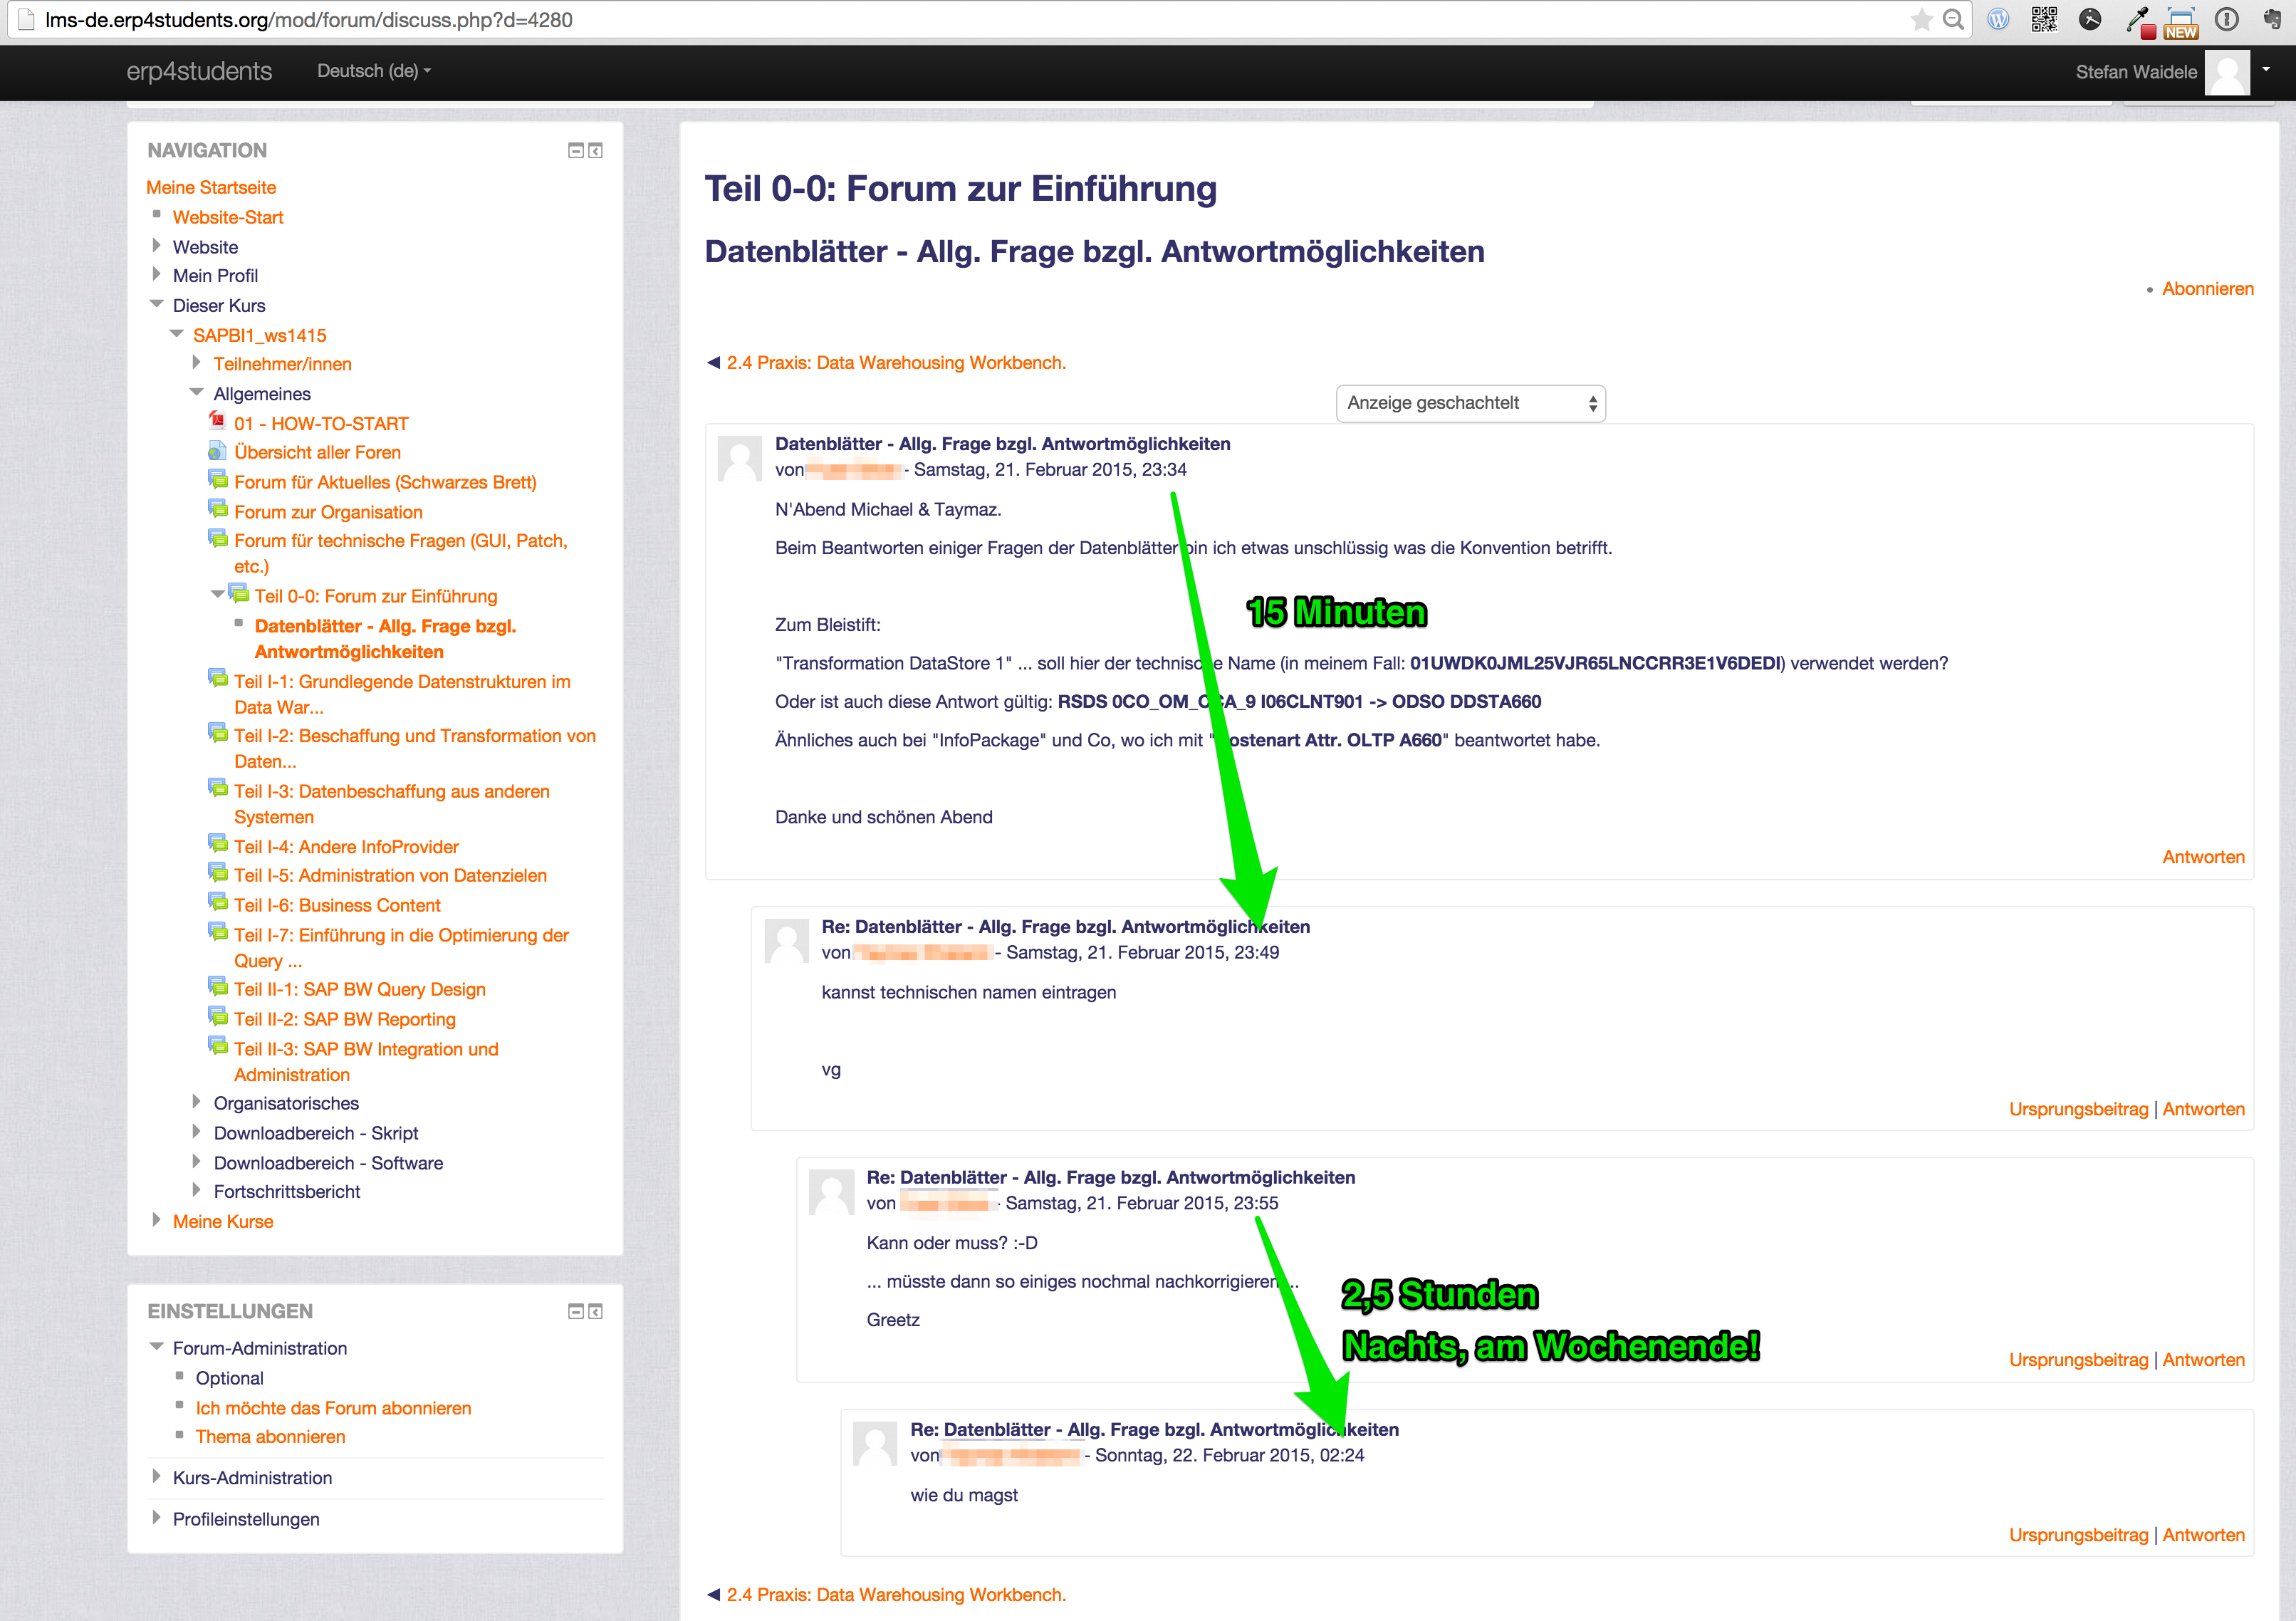
\includegraphics[width=\textwidth]{erp4students.jpg}
\caption{Screenshot: Forum von ERP4students}
\label{fig:erp4s}
\end{center}
\end{figure}

Als negativer Effekt der schnellen Unterstützung durch die Dozenten lässt sich jedoch die geringe Interaktion zwischen den Studierenden bemängeln. In der untersuchten Stichprobe kam nur eine von 53 Antworten von einem Kommilitonen des Fragestellers. Dies ist jedoch aufgrund der hohen Konzentration auf ein bestimmtes Thema und des recht hohen Lernpensum akzeptabel, da die meisten Fragen im Forum in den Bereich „dringend und relevant aber geringes pädagogisches Potential“ nach dem in Abschnitt~\myref{sub:zielkonflikt_betreuungsqualitat_vs_involvement} Schema fallen.\footnote{Screenshot siehe Abbildung~\ref{fig:erp4s} auf Seite~\pageref{fig:erp4s}}
% subsection erp4students (end)

\subsection{Shootcamp.at} % (fold)
\label{sub:shootcamp_at}

Die Foren von \buzz{Shootcamp.at}, einem Online–Kurs für ambitionierte Hobbyfotografen, ergänzen die vom Dozenten bereitgestellten Online–Videos. Da die Fragen in diesem Forum aufgrund des sehr lockeren Zeitplans, dem Fehlen jeglicher Prüfungsleistung und der ständigen Ermutigung des Dozenten, sich Zeit für Experimente zu nehmen nur in den allerwenigsten Fällen als „Dringend“ eingestuft werden können, fällt es nicht negativ auf, dass die Dozentenmeinung hauptsächlich in den Lernvideos und fast nicht im Forum zu finden ist. 

Durch das Fehlen von vorgegebenen Lösungen wird das pädagogische Potential der Gruppendiskussionen und Bildbesprechungen genutzt. Lernende sprechen miteinander über Ideen und Verbesserungsvorschläge, was das Wissen und die Fähigkeiten aller Diskussionsteilnehmer erweitert und vertieft. \footnote{Screenshot siehe Abbildung~\ref{fig:scamp} auf Seite~\pageref{fig:scamp}}
\begin{figure}[p]
\begin{center}
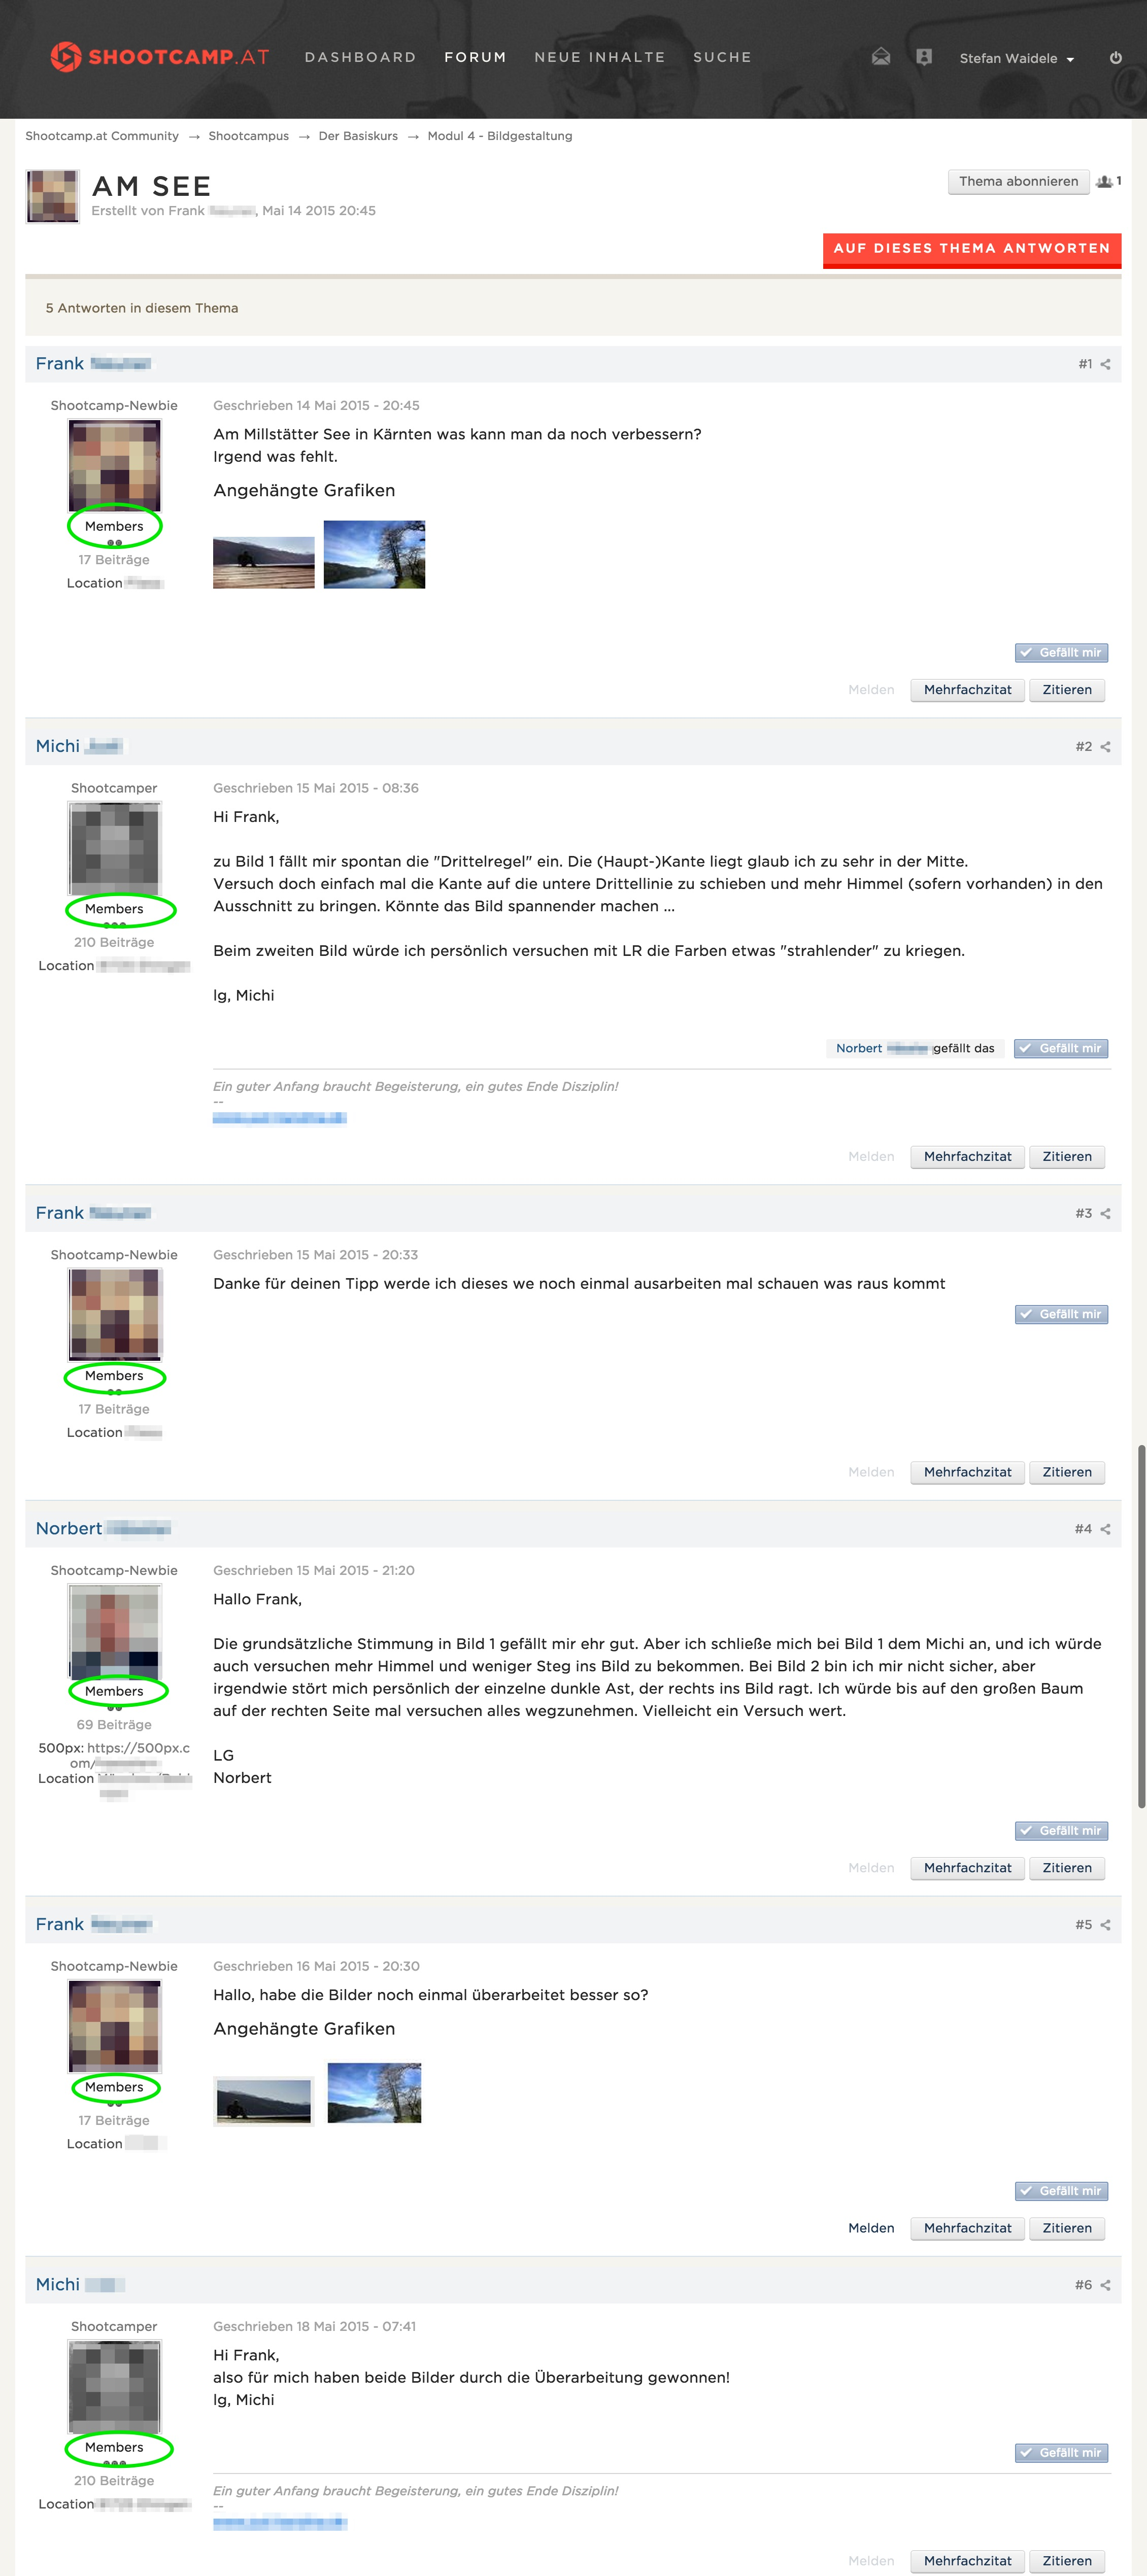
\includegraphics[width=.7\textwidth]{shootcamp.jpg}
\caption{Screenshot: Forum von Shootcamp.at}
\label{fig:scamp}
\end{center}
\end{figure}

% subsection shootcamp_at (end)

\subsection{OnCampus.de: LINAVO} % (fold)
\label{sub:oncampus_de}

Die Online–Kurse von \buzz{\ac{LINAVO}} stützen sich auf Online–Lernunterlagen, wie jedoch durch den jeweiligen Dozenten im Forum durch Links auf aktuelle Artikel und durch Rechercheaufgaben erweitert werden. Die Diskussion zu den Themen wird offen geführt und es wird eine wissenschaftliche Argumentationsweise mit Belegen und Quellenangaben eingefordert. Hierdurch wird das pädagogische Potential auf akademischem Niveau entwickelt.

\begin{figure}[p]
\begin{center}
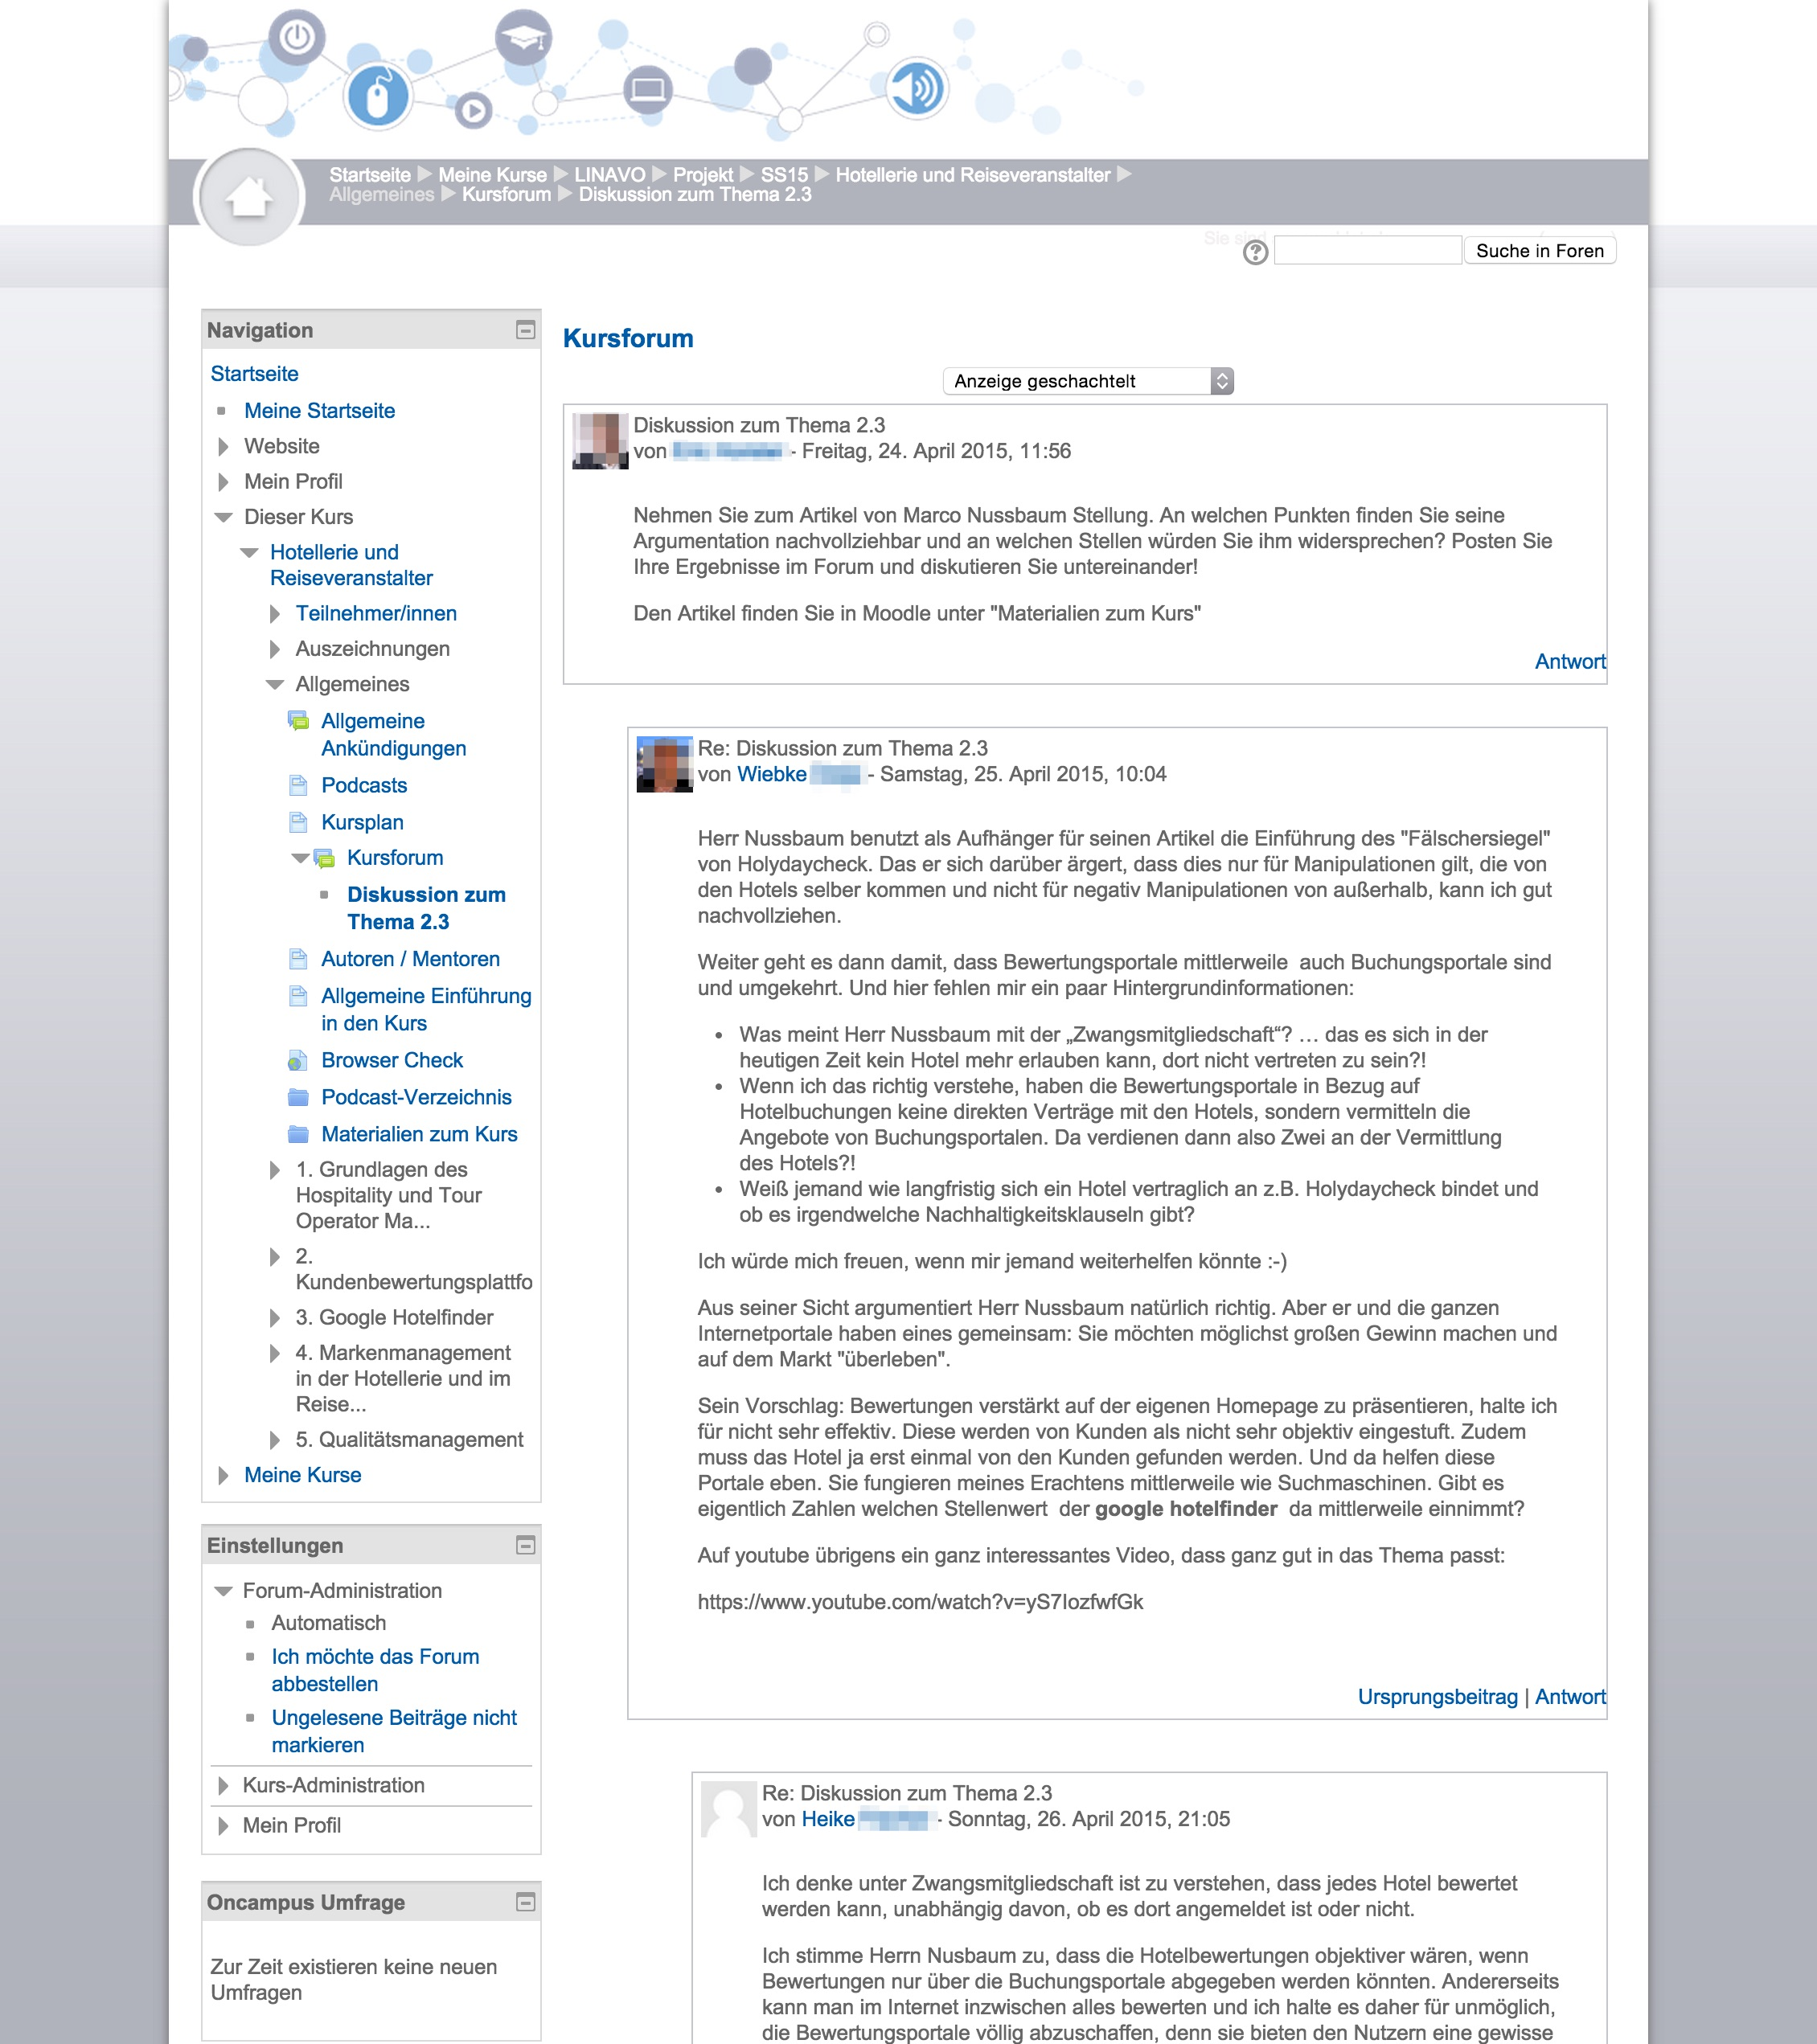
\includegraphics[width=\textwidth]{linavo.jpg}
\caption{Screenshot: Forum von LINAVO}
\label{fig:linavo}
\end{center}
\end{figure}

Aufgrund des akademischen Anspruchs werden z.T. Beiträge im DOC–Format mit entsprechender Formatierung zur Diskussion eingereicht.\footnote{z.B. mit 1,5–fachem Zeilenabstand oder Fußnoten für Quellenangaben} Dies verhindert dann allerdings die Nutzung der Stärken eines Forensystems, wie etwa das direkte Bezugnehmen auf den Gesprächspartner. Außerdem sind zum Download und zur Anzeige von Dateianhängen weitere Arbeitsschritte notwendig.\footnote{Screenshot siehe Abbildung~\ref{fig:linavo} auf Seite~\pageref{fig:linavo}}
% subsection oncampus_de (end)

\subsection{Hasso Plattner Institut: openHPI} % (fold)
\label{sub:hasso_plattner_institut}

Im CSCL–Angebot des Hasso Plattner Instituts \buzz{openHPI} ist die technische Unterstützung explizit an ein von jeder Seite aus erreichbares Helpdesk–System delegiert. Hierdurch werden Probleme mit den System und die akademische Diskussion voneinander getrennt. Forenbeiträge können über ein Abstimmsystem positiv („Upvote“) und negativ („Downvotes“) bewertet werden. Hierdurch kann die Aufmerksamkeit der Tutoren auf diese Beiträge gelenkt werden. Wichtige Diskussionen werden in Dozentenvideos besprochen.\footnote{vgl. \cite{hpiintro}, Abschnitt „Fragen und Probleme“}

Weiterhin können Fragen im Forum von den Teilnehmern entweder „kommentiert“ oder „beantwortet” werden. Diese Unterscheidung ermöglicht es, den eigenen Beiträge eine entsprechende Bedeutung zuzuordnen und dadurch wichtige Beiträge mit vielen Upvotes aber ohne Antworten schnell zu identifizieren und den Dozenten somit Handlungsbedarf anzuzeigen.\footnote{Screenshot siehe Abbildung~\ref{fig:hpi} auf Seite~\pageref{fig:hpi}}

\begin{figure}[p]
\begin{center}
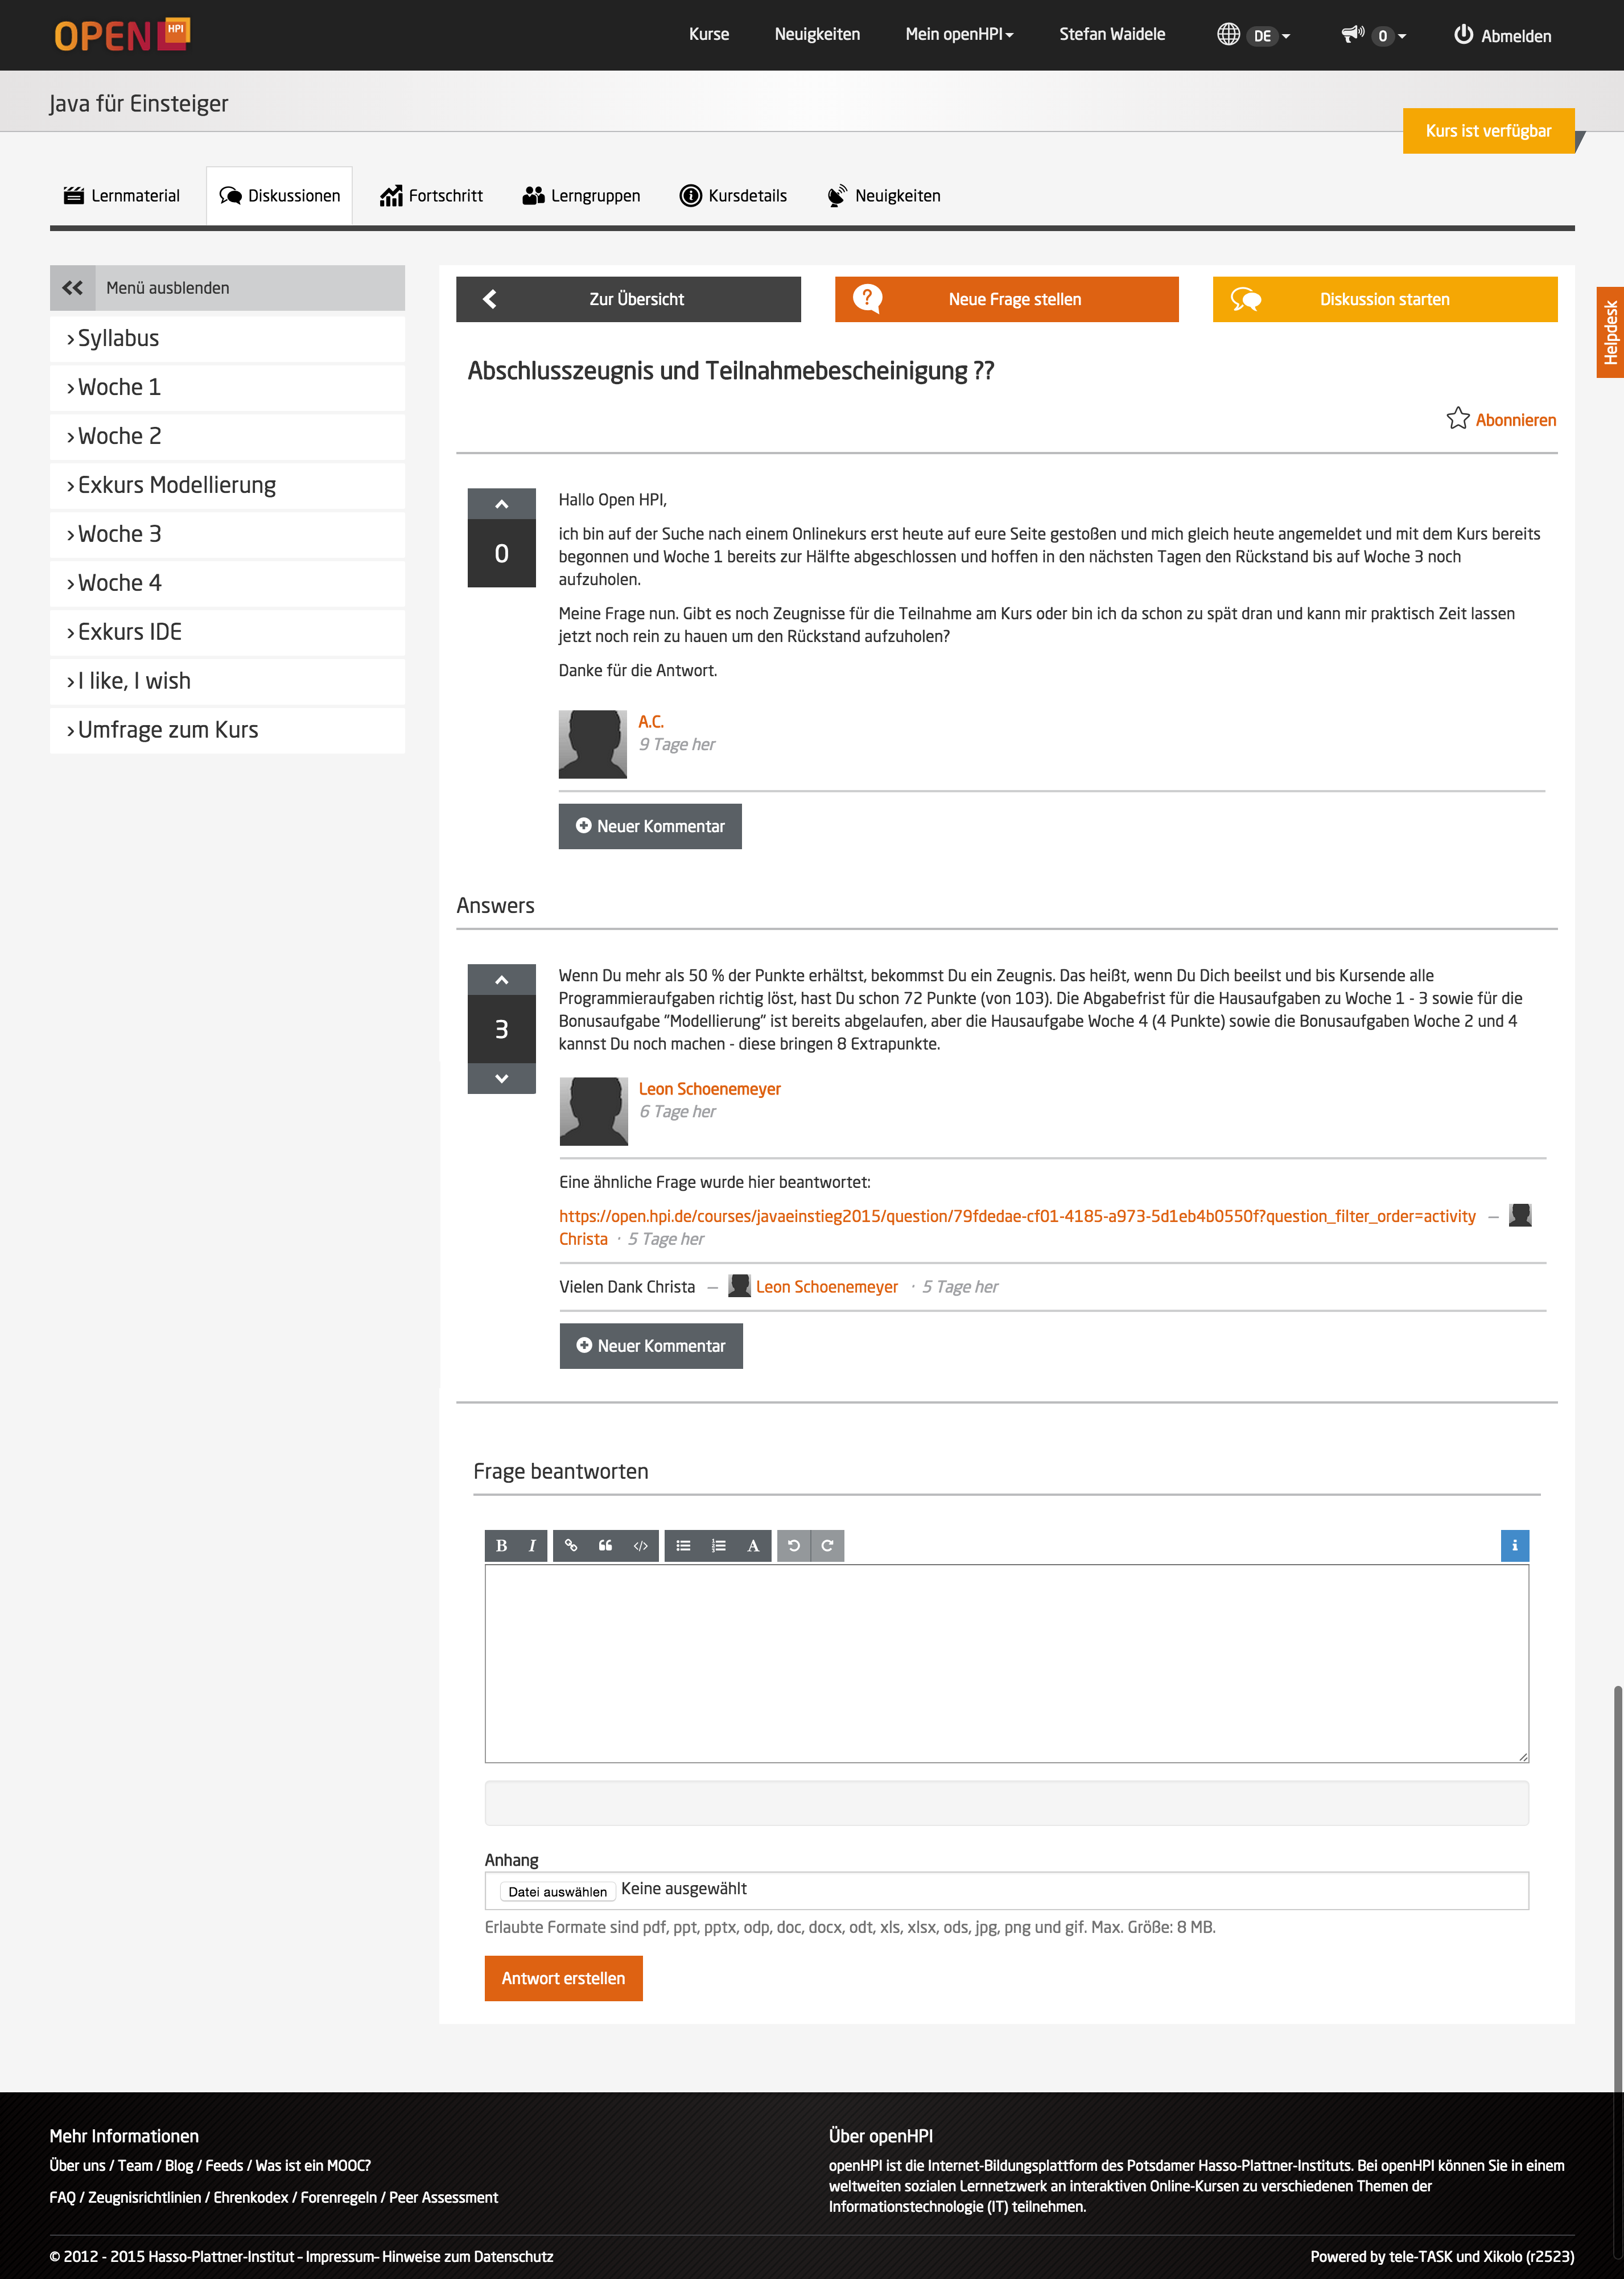
\includegraphics[width=\textwidth]{hpiforum.png}
\caption{Screenshot: Forum des Hasso Plattner Instituts}
\label{fig:hpi}
\end{center}
\end{figure}
% subsection hasso_plattner_institut (end)

\subsection{Anreiz– und Feedbacksysteme} % (fold)
\label{sub:infentives}

Über verschiedene Arten von Anreizsystemen können Teilnehmer dazu gebracht werden, aktiv am gemeinschaftlichen Lernprozess teilzunehmen. Hierzu können einzelne Beiträge positiv (durch klicken von „Gefällt mir.“ oder Ähnlichem\footnote{siehe z.B. \url{Facebook.com} oder \url{ShootCamp.at}}) oder positiv und negativ (durch Up– bzw. Downvotes\footnote{siehe z.B. \url{openHPI} oder \url{StackOverflow.com}}) bewertet werden.

Zusätzlich oder alternativ können auch Teilnehmer ihre digitale Reputation im \ac{CSCL}–System entwickeln. Diese wird in Foren i.d.R. über die Anzahl der geleisteten Beiträge gemessen, die in den entsprechenden Titel umgerechnet werden.\footnote{siehe z.B. \url{Fernstudenten.de}}
% subsection infentives (end)

% section best_practice (end)
